\documentclass[12pt]{article}
\usepackage{geometry}
\usepackage{amsmath}
\usepackage{amssymb}
\usepackage{enumitem}
\usepackage{fancyhdr}
\usepackage{tikz}
\usepackage{graphicx}
\usepackage{xcolor}
\usetikzlibrary{trees}
\pagestyle{fancy}


% \lhead{Problem \arabic{enumi}}
\lhead{Jaykumar Patel}
\chead{Homework 0}
\rhead{EID: jnp2369}

\begin{document}

\title{Homework 0 Solutions}

Collaborators: Boting Lu, Janvi Patel, Aniketh Devarasetty

\section{Multiple Choice}

\subsection{}
A linear equation system Ax = b has a single unique solution if?

A.) A is square

B.) A is symmetric

C.) A is square and full rank

D.) A is square and symmetric

\color{blue}
Answer: C - A is square and full rank

\color{black}
\subsection{}
Given a K-dimensional vector X (i.e., containing K elements), which one of the following operations cannot be represented by a linear transformation AX, with regard to some appropriate matrix A?

A.) Keeping the first three elements of X and discarding others

B.) Amplifying the vector norm of X by two times

C.) In the polar coordinate system, rotating the angle of X by 45 degrees

D.) Sorting all elements by magnitude in the descending order

\color{blue}
Answer: D - Sorting all elements by magnitude in the descending order

\color{black}
\section{Short Answer}

\subsection{}

\subsubsection{}
If $v_1, ..., v_m \in V$ are linearly independent, and $T : V \rightarrow W$ is a linear operator, is it true that $Tv_1, ..., Tv_m \in W$ must be linearly independent? Explain your reasoning.

\color{blue}
Answer: It is not true. Suppose the linear operator $T$ transforms all vectors to the 0 vector. Then, every vector $v_1, ..., v_m \in V$ will get transformed to the 0 vector. Thus, $Tv_1, ..., Tv_m \in W$ will all be 0 vectors. Since any zero vector can be represented as a linear combination of any other zero vectors, $Tv_1, ..., Tv_m \in W$ will not be linearly independent.

\color{black}
\subsubsection{}
If $v_1, ..., v_m \in V$ are dependent, and $T : V \rightarrow W$ is a linear operator, is it true that $Tv_1, ..., Tv_m \in W$ must be dependent? Explain your reasoning.

\color{blue}
Answer: Yes this is true. If $v_1, ..., v_m \in V$ are dependent, then there exist a subset of vectors $v_x, v_y, ..., v_z \in V$ such that $\alpha v_x + \beta v_y + ... + \lambda v_z = 0$ where at least 1 of the coefficients (out of $\alpha, \beta, ..., \lambda$) are non-zero. Applying the linear transformation T, we get the following:

\begin{align*}
&\alpha v_x + \beta v_y + ... + \lambda v_z = 0 \\
&T(\alpha v_x + \beta v_y + ... + \lambda v_z) = T(0) \\
&T(\alpha v_x) + T(\beta v_y) + ... + T(\lambda v_z) = 0 \\
&\text {Since T is a linear operator, we can factor out the coefficients} \\
&\alpha T(v_x) + \beta T(v_y) + ... + \lambda T(v_z) = 0 \\
\end{align*}

Since at least 1 of the coefficients are non-zero for the equation $\alpha T(v_x) + \beta T(v_y) + ... + \lambda T(v_z) = 0$, we can conclude that $Tv_1, ..., Tv_m \in W$ is dependent.

\color{black}
\subsection{}
Hand-compute the euclidean distance of the following two vectors: $\vec{a} = [10,20,15,10,5]$, $\vec{b} = [12,24,18,8,7]$. Please write down your computation process.

\color{blue}
Answer: Suppose $d(\vec{a}, \vec{b})$ represents the euclidean distance between $\vec{a}$ and $\vec{b}$.

\begin{align*}
d(\vec{a}, \vec{b}) &= \sqrt{(12 - 10)^2 + (24 - 20)^2 + (18 - 15)^2 + (8 - 10)^2 + (7 - 5)^2} \\
&= \sqrt{2^2 + 4^2 + 3^2 + (-2)^2 + 2^2} \\
&= \sqrt{4 + 16 + 9 + 4 + 4} \\
&= \sqrt{37}
\end{align*}

\color{black}
\subsection{}

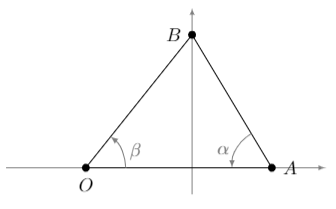
\includegraphics{images/2-3-Triangle.png}

\subsubsection{}
Express $|OA|$ (the vector norm, or length) using $|OB|$, $|AB|$, $\alpha$ and $\beta$. Hint: use projections.

\color{blue}
Answer: Consider the vertical line that goes through $B$ and intersects line $OA$ perpendicularily. Consider this point of intersection on line $OA$ as $\Theta$. Thus, $|O \Theta| + |\Theta A| = |OA|$.

Given the above premise, we can calculate $|OA|$ using the following logic:

\begin{align*}
cos(\beta) &= \frac{|O \Theta}{|OB|} \rightarrow |O \Theta| = cos(\beta) \cdot |OB| \\
cos(\alpha) &= \frac{|\Theta A|}{|AB|} \rightarrow |\Theta A| = cos(\alpha) \cdot |AB| \\
|OA| &= |O \Theta| + |\Theta A| \\
&= (cos(\beta) \cdot |OB|) + (cos(\alpha) \cdot |AB|)
\end{align*}

\color{black}
\subsubsection{}
Express $|AB|$ using $|OB|$, $|OA|$, and $\beta$.

\color{blue}
Answer: Using the Law of Cosines, we get the following:
\begin{align*}
|AB| = \sqrt{|OB|^2 + |OA|^2 - 2|OB||OA|cos(\beta)}
\end{align*}

\color{black}
\subsection{}
Hand-compute the matrix-vector product: $B = A\vec{x}$, where $A = $
$\begin{bmatrix}
    1 & -1 & 2 \\
    0 & -3 & 1
\end{bmatrix}$
and $\vec{x} = $
$\begin{bmatrix}
    5 \\
    7 \\
    1
\end{bmatrix}$
.

\color{blue}
Answer:
\begin{align*}
    B &= A\vec{x} \\
    &=
    \begin{bmatrix}
        1 & -1 & 2 \\
        0 & -3 & 1
    \end{bmatrix}
    \begin{bmatrix}
        5 \\
        7 \\
        1
    \end{bmatrix} \\
    &=
    \begin{bmatrix}
        (1)(5) + (-1)(7) + (2)(1) \\
        (0)(5) + (-3)(7) + (1)(1)
    \end{bmatrix} \\\
    &=
    \begin{bmatrix}
        0 \\
        -20
    \end{bmatrix}
\end{align*}

\color{black}
\subsection{}
A sample sequence $x(n)$ is shown in Figure 1. The unit impulse signal is denoted by $\delta(n)$ and is defined as $\delta(n) = \lbrace 1 \text{ for } n = 0, 0 \text{ for } n \neq 0 \rbrace $. Express $x(n)$ as a linear combination of weighted and delayed unit samples.

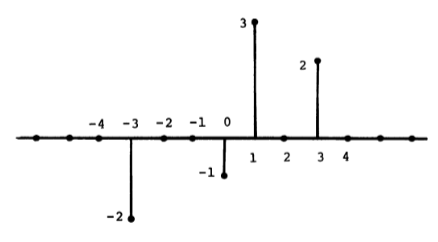
\includegraphics{images/2-5-Signal.png}

\color{blue}
Answer: $x(n) = -2 \delta(n + 3) - \delta(n) + 3 \delta(n - 1) + 2 \delta(n - 3)$

\color{black}
\subsection{}
Hand-compute eigenvalues of the following matrix:
$\begin{bmatrix}
    0 & 1 \\
    -2 & -3
\end{bmatrix}$
. Please write down your computation process.

\color{blue}
Answer: Suppose that $\lambda$ represents the eigenvalues. Then:
\begin{align*}
    A &= 
    \begin{bmatrix}
        0 & 1 \\
        -2 & -3
    \end{bmatrix} \\
    I &=
    \begin{bmatrix}
        1 & 0 \\
        0 & 1
    \end{bmatrix} \\
    A - \lambda I &=
    \begin{bmatrix}
        0 & 1 \\
        -2 & -3
    \end{bmatrix}
    -
    \begin{bmatrix}
        \lambda & 0 \\
        0 & \lambda
    \end{bmatrix} \\
    &=
    \begin{bmatrix}
        - \lambda & 1 \\
        -2 & -3 - \lambda
    \end{bmatrix} \\
    |A - \lambda I| &= |
    \begin{bmatrix}
        - \lambda & 1 \\
        -2 & -3 - \lambda
    \end{bmatrix}
    | \\
    &= (- \lambda)(-3 - \lambda) - (1)(-2) \\
    &= (3 \lambda + \lambda^2) + 2 \\
    &= \lambda^2 + 3 \lambda + 2 \\
    &= (\lambda + 1) (\lambda + 2) \\
    \lambda &= -1 \\
    \lambda &= -2
\end{align*}

Thus, the eigenvalues of matrix
$\begin{bmatrix}
    0 & 1 \\
    -2 & -3
\end{bmatrix}$
are $-1$ and $-2$.

\color{black}

\end{document}